\documentclass[12pt]{exam}

% essential packages
\usepackage{fullpage} % margin formatting
\usepackage{enumitem} % configure enumerate and itemize
\usepackage{amsmath, amsfonts, amssymb, mathtools} % math symbols
\usepackage{xcolor, colortbl} % colors, including in tables
\usepackage{makecell} % thicker \Xhline in table
\usepackage{graphicx} % images, resizing

\usepackage[dvipsnames]{xcolor}
\usepackage[framemethod=tikz]{mdframed}

\newcommand{\commentsection}[1]{
  \begin{mdframed}[roundcorner=10pt,leftmargin=1cm,%
                     rightmargin=1cm,backgroundcolor=SkyBlue!20,%
                     innertopmargin=\baselineskip,%
                     skipabove=\baselineskip,%
                     skipbelow=\baselineskip]
  #1
  \end{mdframed}
}

% sometimes needed packages
\usepackage{hyperref} % hyperlinks
% \hypersetup{colorlinks=true, urlcolor=blue}
% \usepackage{logicproof} % natural deduction
% \usepackage{tikz} % drawing graphs
% \usetikzlibrary{positioning}
% \usepackage{multicol}
% \usepackage{algpseudocode} % pseudocode

% paragraph formatting
\setlength{\parskip}{6pt}
\setlength{\parindent}{0cm}

% newline after Solution:
\renewcommand{\solutiontitle}{\noindent\textbf{Solution:}\par\noindent}


% less space before itemize/enumerate
\setlist{topsep=0pt}

% creates \filcl to grey out cells for groupwork grading
\newcommand{\filcl}{\cellcolor{gray!25}}

% creates \probnum to get the problem number
\newcounter{probnumcount}
\setcounter{probnumcount}{1}
\newcommand{\probnum}{\arabic{probnumcount}. \addtocounter{probnumcount}{1}}

% use roman numerals by default
\setlist[enumerate]{label={(\roman*)}}

% creates custom list environments for grading guidelines, question parts
\newlist{guidelines}{itemize}{1}
\setlist[guidelines]{label={}, left=0pt .. \parindent, nosep}
\newlist{gwguidelines}{enumerate}{1}
\setlist[gwguidelines]{label={(\roman*)}, nosep}
\newlist{qparts}{enumerate}{2}
\setlist[qparts]{label={(\alph*)}}
\newlist{qsubparts}{enumerate}{2}
\setlist[qsubparts]{label={(\roman*)}}
\newlist{stmts}{enumerate}{1}
\setlist[stmts]{label={(\roman*)}, nosep}
\newlist{pflist}{itemize}{4}
\setlist[pflist]{label={$\bullet$}, nosep}
\newlist{enumpflist}{enumerate}{4}
\setlist[enumpflist]{label={(\arabic*)}, nosep}

\printanswers

\newcommand{\prevhwnum}{5}
\newcommand{\hwnum}{5}

\begin{document}
\pagebreak

\section*{Grading of Groupwork \prevhwnum{}}
Using the solutions and Grading Guidelines, grade your Groupwork \prevhwnum{} Problems:
\begin{itemize}
    \item Use the table below to grade your past groupwork submission and calculate scores.
    \item While grading, mark up your past submission. Include this with the table when you submit your grading.
    \item Write whether your submission achieved each rubric item. If it didn't achieve one, say why not.
    \item For extra credit, write positive comment(s) about your work.
    \item You don't have to redo problems correctly, but it is recommended!
    \item See ``All About Groupwork" on Canvas for more detailed guidance, and what to do if you change groups.
\end{itemize}

\begin{center}
\resizebox{\textwidth}{!}{\begin{tabular}{| c | c | c | c | c | c | c | c | c | c | c | c | c |}
\hline
 & (i) & (ii) & (iii) & (iv) & (v) & (vi) & (vii) & (viii) & (ix) & (x) & (xi) & Total:\\
\hline
Problem 1 & & & & & & &\filcl &\filcl &\filcl & \filcl& \filcl& \hspace{1cm}/12\\
\hline 
Problem 2 & & & & & & &\filcl &\filcl &\filcl & \filcl& \filcl& \hspace{1cm}/18\\
\Xhline{1.25pt}
Total: &\filcl &\filcl &\filcl &\filcl &\filcl &\filcl &\filcl &\filcl & \filcl& \filcl& \filcl&\hspace{1cm}/30\\
\hline
\end{tabular}}
\end{center}
\section*{Comments}


\commentsection{I don't really get the second problem. However, I figured out the first problem on my own, kuddos to me.}
\setcounter{probnumcount}{1}
\section*{Groupwork \hwnum{} Problems}

\subsection*{\probnum Plane Cutting [12 points]}
If $n$ lines are drawn on a plane, no two lines are parallel, and all pairs of lines intersect at different points, how many sections do they separate the plane into? Assume that no more than two lines intersect at any one point.  Prove your result using weak induction. Don't include unneeded base cases.

\begin{solution}
	\begin{tabular}{ll}
		Proof:                                                                                       \\
		Proof by weak induction.                                                                     \\
		Let $P(n)$ be the statement that $n$ lines drawn on a plane separate the plane               \\
		into $\frac{n(n+1)}{2}+1$ sections.                                                          \\
		Let $k\in \mathbb{Z}^+, k\ge 1, k$ be arbitary                                               \\
		Inductive step:                                                                              \\
		Assume $P(k)$.                                                                               \\
		Want to show: $P(k+1)$                                                                       \\
		Take a plane with $k$ lines.                                                                 \\
		Add a new line.                                                                              \\
		This new line intersects the $k$ lines at $k$ different points.                              \\
		This new line separates the plane into $k+1$ new sections.                                   \\
		Thus, the total number of sections is:                                                       \\
		$\frac{k(k+1)}{2}+1+k+1=\frac{k^2+k+2k+2}{2}+1=\frac{k^2+3k+2}{2}+1=\frac{(k+1)(k+2)}{2}+1$. \\
		Since $P(k+1)$ holds, $P(n)$ is true for all positive integers $n$.                          \\
		Base case:                                                                                   \\
		LHS:                                                                                         \\
		$P(1)=\frac{1(1+1)}{2}+1=2$                                                                  \\
		RHS:                                                                                         \\
		$P(1)=P(0)+1=1+1=2$                                                                          \\
	\end{tabular}
	\\Thus, by weak induction, $P(n)$ is true for all positive integers $n$.
\end{solution}

\subsection*{\probnum Splitting Stones [18 points]}
In front of you sits a pile of $n$ stones.  You split the pile into two smaller piles, count the number of stones in the smaller pile, $j$, and write down the number $2^j$. Then, for each of the two piles, you split them and write down their versions of $2^j$.  You repeat this process, splitting piles and writing down exponentials until all piles have only 1 stone in them.  Finally, you multiply together all the numbers you wrote down.

For example, if we start with 8 stones, one possible way these piles could be split is as follows:

\begin{center}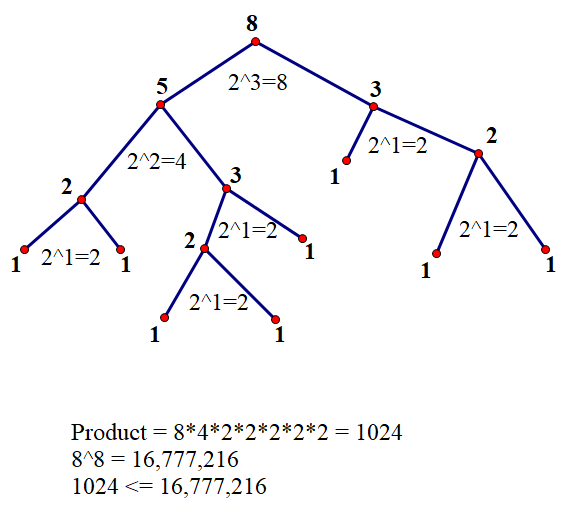
\includegraphics[scale=.75]{induction.png}\end{center}

Prove using strong induction that no matter how you split the piles, the overall product you get is less than or equal to $n^ n$.

\textbf{Hint:} When there is only one stone, you cannot split the pile, and the process stops.

\begin{solution}

	\begin{tabular}{ll}
		Proof:                                                                                   \\
		Proof by strong induction.                                                               \\
		Let $P(n)$ be the statement that the overall product is less than or equal to $n^n$.     \\
		Let $k\in \mathbb{Z}^+, k\ge 1, k$ be arbitary                                           \\
		Inductive step:                                                                          \\
		Assume $P(j), \forall j(1\le j\le k-1)$                                                  \\
		Want to show: $P(k)$                                                                     \\
		Take a pile of $k$ stones.                                                               \\
		Split the pile into two smaller piles.                                                   \\
		Let $i$ be the number of stones in the smaller pile.                                     \\
		Since $i\le k-1$, by I.H., the overall product of the smaller pile is $\le (k-1)^{k-1}$. \\
		The overall product of the larger pile is $\le (k-i)^{k-i}$.                             \\
		The overall product of the pile of $k$ stones is $\le i^{i}\cdot (k-i)^{k-i}$.           \\
		Since $i\le k-1$, $i^{i}\le (k-1)^{k-1}$.                                                \\
		Thus, the overall product of the pile of $k$ stones is:                                  \\
		$\le (k-1)^{k-1}\cdot (k-1)^{k-1}=(k-1)^{k-1}\cdot (k-1)^{k-1}=(k-1)^{k}$.               \\
		Since $P(k)$ holds, $P(n)$ is true for all positive integers $n$.                        \\
		Base case:                                                                               \\
		$P(1)=1^1=1$                                                                             \\
		Thus, by strong induction, $P(n)$ is true for all positive integers $n$.
	\end{tabular}
\end{solution}
\end{document}
